\pdfoptionpdfminorversion=4

%%%%%%%%%%%%%%%%%%%%%%%%%%%%%%%%%%%%%%%%%%%%%%%%%%%%%%%%%%%%%%%%%%%%%
%% This is a (brief) model paper using the achemso class
%% The document class accepts keyval options, which should include
%% the target journal and optionally the manuscript type.
%%%%%%%%%%%%%%%%%%%%%%%%%%%%%%%%%%%%%%%%%%%%%%%%%%%%%%%%%%%%%%%%%%%%%
\documentclass[journal=jpcbfk,manuscript=suppinfo,layout=traditional]{achemso}

%%%%%%%%%%%%%%%%%%%%%%%%%%%%%%%%%%%%%%%%%%%%%%%%%%%%%%%%%%%%%%%%%%%%%
%% Place any additional packages needed here.  Only include packages
%% which are essential, to avoid problems later.
%%%%%%%%%%%%%%%%%%%%%%%%%%%%%%%%%%%%%%%%%%%%%%%%%%%%%%%%%%%%%%%%%%%%%
\usepackage{chemformula} % Formula subscripts using \ch{}
\usepackage[T1]{fontenc} % Use modern font encodings
\usepackage{graphicx}
\usepackage{caption}
\usepackage{amsmath}
\usepackage{mathptmx}
\usepackage{multirow}
\usepackage{tabularx,booktabs}
\usepackage{color, colortbl}
\usepackage{subcaption}
\usepackage[scaled=0.92]{helvet}
%%%%%%%%%%%%%%%%%%%%%%%%%%%%%%%%%%%%%%%%%%%%%%%%%%%%%%%%%%%%%%%%%%%%%
%% If issues arise when submitting your manuscript, you may want to
%% un-comment the next line.  This provides information on the
%% version of every file you have used.
%%%%%%%%%%%%%%%%%%%%%%%%%%%%%%%%%%%%%%%%%%%%%%%%%%%%%%%%%%%%%%%%%%%%%
%%\listfiles

%%%%%%%%%%%%%%%%%%%%%%%%%%%%%%%%%%%%%%%%%%%%%%%%%%%%%%%%%%%%%%%%%%%%%
%% Place any additional macros here.  Please use \newcommand* where
%% possible, and avoid layout-changing macros (which are not used
%% when typesetting).
%%%%%%%%%%%%%%%%%%%%%%%%%%%%%%%%%%%%%%%%%%%%%%%%%%%%%%%%%%%%%%%%%%%%%
\newcommand*\mycommand[1]{\texttt{\emph{#1}}}

%%%%%%%%%%%%%%%%%%%%%%%%%%%%%%%%%%%%%%%%%%%%%%%%%%%%%%%%%%%%%%%%%%%%%
%% Meta-data block
%% ---------------
%% Each author should be given as a separate \author command.
%%
%% Corresponding authors should have an e-mail given after the author
%% name as an \email command. Phone and fax numbers can be given
%% using \phone and \fax, respectively; this information is optional.
%%
%% The affiliation of authors is given after the authors; each
%% \affiliation command applies to all preceding authors not already
%% assigned an affiliation.
%%
%% The affiliation takes an option argument for the short name.  This
%% will typically be something like "University of Somewhere".
%%
%% The \altaffiliation macro should be used for new address, etc.
%% On the other hand, \alsoaffiliation is used on a per author basis
%% when authors are associated with multiple institutions.
%%%%%%%%%%%%%%%%%%%%%%%%%%%%%%%%%%%%%%%%%%%%%%%%%%%%%%%%%%%%%%%%%%%%%
\author{Sree Ganesh Balasubramani}
\affiliation{Department of Chemistry and Biochemistry, University of Arizona, Tucson, Arizona 85721, United States}
\author{Steven D. Schwartz}
\affiliation{Department of Chemistry and Biochemistry, University of Arizona, Tucson, Arizona 85721, United States}
%\author{I. Ken Groupleader}
%\altaffiliation{A shared footnote}
\email{sschwartz@email.arizona.edu}
%\phone{+123 (0)123 4445556}
%\fax{+123 (0)123 4445557}
%\affiliation[Unknown University]
%{Department of Chemistry, Unknown University, Unknown Town}
%\alsoaffiliation[Second University]
%{Department of Chemistry, Second University, Nearby Town}

%%%%%%%%%%%%%%%%%%%%%%%%%%%%%%%%%%%%%%%%%%%%%%%%%%%%%%%%%%%%%%%%%%%%%
%% The document title should be given as usual. Some journals require
%% a running title from the author: this should be supplied as an
%% optional argument to \title.
%%%%%%%%%%%%%%%%%%%%%%%%%%%%%%%%%%%%%%%%%%%%%%%%%%%%%%%%%%%%%%%%%%%%%
\title[]
  {Transition path sampling based calculations of free energies for enzymatic
  reactions: the case of human methionine adenosyl transferase and plasmodium 
  vivax adenosine deaminase}
%%%%%%%%%%%%%%%%%%%%%%%%%%%%%%%%%%%%%%%%%%%%%%%%%%%%%%%%%%%%%%%%%%%%%
%% Some journals require a list of abbreviations or keywords to be
%% supplied. These should be set up here, and will be printed after
%% the title and author information, if needed.
%%%%%%%%%%%%%%%%%%%%%%%%%%%%%%%%%%%%%%%%%%%%%%%%%%%%%%%%%%%%%%%%%%%%%
\abbreviations{TPS,WHAM}
\keywords{American Chemical Society, \LaTeX}

%%%%%%%%%%%%%%%%%%%%%%%%%%%%%%%%%%%%%%%%%%%%%%%%%%%%%%%%%%%%%%%%%%%%%
%% The manuscript does not need to include \maketitle, which is
%% executed automatically.
%%%%%%%%%%%%%%%%%%%%%%%%%%%%%%%%%%%%%%%%%%%%%%%%%%%%%%%%%%%%%%%%%%%%%
\begin{document}

%%%%%%%%%%%%%%%%%%%%%%%%%%%%%%%%%%%%%%%%%%%%%%%%%%%%%%%%%%%%%%%%%%%%%
%% The "tocentry" environment can be used to create an entry for the
%% graphical table of contents. It is given here as some journals
%% require that it is printed as part of the abstract page. It will
%% be automatically moved as appropriate.
%%%%%%%%%%%%%%%%%%%%%%%%%%%%%%%%%%%%%%%%%%%%%%%%%%%%%%%%%%%%%%%%%%%%%
%\begin{tocentry}
\section{\textit{pv}ADA catalyzed reaction}
The reaction catalyzed by \textit{pv}ADA is between adenosine and OH$^{-}$ anion resulting
in the formation of inosine. Experimental studies suggest that the GLU 229 residue 
protonates the N1 atom of the adenosyl moeity and this transfer of proton is almost complete 
at the transition state. \cite{Luo07JAmChemSoc129p8008} The protonation of the N1 atom 
as observed in a representative reactive trajectory from the TPS ensemble is shown in 
Fig. \ref{sfig:he2time}. The dynamics of the proton transfer from the OH group to the 
NH$_2$ group which are both bonded to the adenosine moeity forming a Meissenheimer complex is 
depicted in Fig. \ref{sfig:n6proton}. 

\begin{figure}
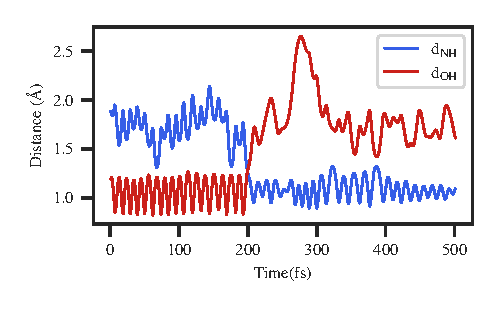
\includegraphics[scale=1]{figures/ada-ohe-nhe60.pdf}
\caption{The distance between the N1-HE2 atoms (d$_{\text{NH}}$) and the OE2-HE2 atoms 
(d$_{\text{OH}}$)in {\AA} as a function of time. The proton is 
transferred from the GLU 229 residue onto the N1 atom of the adenosyl moeity.}
\label{sfig:he2time}
\end{figure}

\begin{figure}
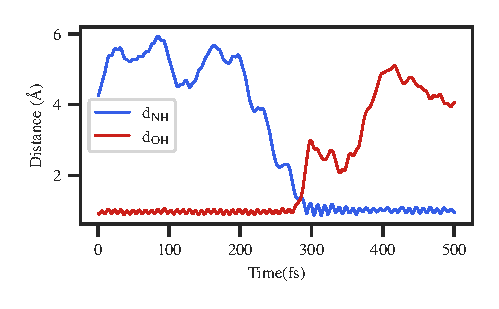
\includegraphics[scale=1]{figures/ada-oh-nh60.pdf}
\caption{The distance between the N6-H1 atoms and O1-H1 atoms as a function of time. The proton transfer from the hydroxide
anion to the NH$_2$ group occurs after the nucleophilic attack of the O1 atom on the C6 atom.}
\label{sfig:n6proton}
\end{figure}

\section{Transition state ensemble for MAT2A enzyme}
\begin{table*}[ht!]
\caption{Order parameters d$_{\text{SC}}$ and d$_{\text{OC}}$ in {\AA} for the 11 transition states obtained from 
the TPS ensemble along with the mean and standard deviation (Stddev).}
\centering
\begin{tabular}{l c c}
\hline\hline
Transition state & d$_{\text{SC}}$ ({\AA}) & d$_{\text{OC}}$ ({\AA})\\
\hline
1 & 2.30 & 2.10 \\
2 & 2.31 & 2.08 \\
3 & 2.31 & 2.09 \\
4 & 2.34 & 2.14 \\
5 & 2.35 & 2.17 \\
6 & 2.41 & 2.16 \\
7 & 2.41 & 2.11 \\
8 & 2.40 & 2.15 \\
9 & 2.35 & 2.13 \\
10& 2.38 & 2.12 \\
11& 2.29 & 2.06 \\
\hline
Mean & 2.35 & 2.12 \\
Stddev & 0.04 & 0.03 \\
\hline\hline
\end{tabular}
%
\end{table*}


\section{Transition state ensemble for \textit{pv}ADA enzyme}
\begin{table*}[ht!]
\caption{Order parameters d$_{\text{OC}}$ and d$_{\text{NC}}$ in {\AA} for the 11 transition states obtained from 
the TPS ensemble along with the mean and standard deviation (Stddev).}
\centering
\begin{tabular}{l c c}
\hline\hline
Transition state & d$_{\text{OC}}$ ({\AA})& d$_{\text{NC}}$ ({\AA})\\
\hline
1& 1.48  &1.60 \\
2& 1.45  &1.51 \\
3& 1.48  &1.58 \\
4& 1.5   &1.57 \\
5& 1.55  &1.55 \\
6& 1.55  &1.64 \\
7& 1.52  &1.63 \\
8& 1.52  &1.68 \\
9& 1.49  &1.52 \\
10&1.50  &1.64 \\
11&1.49  &1.62 \\
\hline
Mean & 1.50 & 1.59 \\
Stddev & 0.03 & 0.05 \\
\hline\hline
\end{tabular}
%
\end{table*}

%\section{Bootstrapping analysis of the free energy curves}

\bibliography{si}

\end{document}